\documentclass[11pt,a4paper]{article}
\usepackage[T1]{fontenc}
\usepackage[utf8]{inputenc}
\usepackage{lmodern}
\usepackage{amsmath,amssymb,amsthm,mathtools,mathrsfs}
\usepackage{graphicx,float,xcolor,multicol}
\usepackage[shortlabels]{enumitem}
\usepackage[margin=27mm]{geometry}
\usepackage{microtype,needspace,placeins}
\usepackage{tikz,tikz-cd}
\usetikzlibrary{arrows.meta,calc,positioning,patterns,decorations.pathreplacing}
\usepackage[colorlinks=true,linkcolor=teal,urlcolor=teal,citecolor=teal]{hyperref}
\setlength{\parindent}{0pt}
\setlength{\parskip}{.6em}
\setcounter{secnumdepth}{0}
\allowdisplaybreaks
\raggedbottom
\providecommand{\cross}{\times}
\DeclareUnicodeCharacter{2020}{\ensuremath{\dagger}}
\DeclareMathOperator{\supp}{supp}
\DeclareMathOperator*{\esssup}{ess\,sup}
\providecommand{\chapter}{\section}
\newenvironment{tool}[2]{\subsection*{Tool #1 --- #2}}{}
\newcommand{\ToolRef}[1]{Tool #1}
\newcommand{\FigureTag}[2]{\textit{Figure #1}}
\newcommand{\Result}[1]{\subsection*{#1}}
\newcommand{\Application}[1]{\subsubsection*{Application\if\relax\detokenize{#1}\relax\else\space--- #1\fi}}
\newcommand{\ProofHeading}{\par\textit{Proof.}\space}
\newcommand{\ProofOf}[1]{\par\textit{Proof of #1.}\space}
\newcommand{\RemarkHeading}{\par\textbf{Remark.}\space}
\newcommand{\NoteHeading}{\par\textbf{Note.}\space}
\newcommand{\ExerciseHeading}{\par\textbf{Exercise.}\space}

% Rendering support only; mathematical text is in each independent post.
\usepackage{booktabs,array,longtable}
\definecolor{HandoutBlue}{HTML}{2F6690}
\definecolor{HandoutNavy}{HTML}{17365D}
\newtheorem{theorem}{Theorem}
\newtheorem{lemma}[theorem]{Lemma}
\newtheorem{proposition}[theorem]{Proposition}
\newtheorem{corollary}[theorem]{Corollary}
\newtheorem{conjecture}[theorem]{Conjecture}
\newtheorem{definition}{Definition}
\newtheorem{example}{Example}
\newtheorem{namedtoolcounter}{Tool}
\newenvironment{namedtool}[1]{\begin{namedtoolcounter}[#1]}{\end{namedtoolcounter}}
\newtheorem*{claim}{Claim}
\newtheorem*{remark}{Remark}
\newtheorem*{exercise}{Exercise}
\newtheorem*{question}{Question}
\newtheorem*{observation}{Observation}
\newcommand{\SourceChapter}[2]{\section*{#2}}
\newcommand{\Lecture}[2]{\section*{Lecture #1: #2}}
\newcommand{\unclear}[1]{\textit{[unclear: #1]}}
\newcommand{\sourcegap}{\textit{[unfinished in the source]}}
\DeclareMathOperator{\dist}{dist}
\DeclareMathOperator{\id}{id}
\DeclareMathOperator{\Hol}{Hol}
\DeclareMathOperator{\Per}{Per}
\DeclareMathOperator{\Fix}{Fix}
\DeclareMathOperator{\diam}{diam}
\DeclareMathOperator{\Var}{Var}
\DeclareMathOperator{\Leb}{Leb}
\DeclareMathOperator{\Hom}{Hom}
\DeclareMathOperator{\End}{End}
\DeclareMathOperator{\Ann}{Ann}
\DeclareMathOperator{\Spec}{Spec}
\DeclareMathOperator{\Max}{Max}
\DeclareMathOperator{\Ob}{Ob}
\DeclareMathOperator{\Tor}{Tor}
\DeclareMathOperator{\Ass}{Ass}
\DeclareMathOperator{\Mor}{Mor}
\DeclareMathOperator{\Fun}{Fun}
\DeclareMathOperator{\Nat}{Nat}
\DeclareMathOperator{\Cone}{Cone}
\DeclareMathOperator{\MCG}{MCG}
\DeclareMathOperator{\Aut}{Aut}
\DeclareMathOperator{\Deck}{Deck}
\DeclareMathOperator{\SL}{SL}
\DeclareMathOperator{\PSL}{PSL}
\DeclareMathOperator{\Area}{Area}
\DeclareMathOperator{\im}{im}
\DeclareMathOperator{\PSh}{PSh}
\newcommand{\CRing}{\mathsf{CRings}}
\newcommand{\AMod}{A\text{-}\mathsf{Mod}}
\newcommand{\Ab}{\mathsf{Ab}}
\newcommand{\Z}{\mathbb Z}
\newcommand{\Q}{\mathbb Q}
\newcommand{\R}{\mathbb R}
\newcommand{\C}{\mathbb C}
\newcommand{\N}{\mathbb N}
\newcommand{\kk}{\mathbb k}
\renewcommand{\aa}{\mathfrak a}
\newcommand{\bb}{\mathfrak b}
\newcommand{\pp}{\mathfrak p}
\newcommand{\qq}{\mathfrak q}
\newcommand{\mm}{\mathfrak m}
\newcommand{\nn}{\mathfrak n}
\newcommand{\rad}{\mathrm r}
\newcommand{\cat}[1]{\mathsf{#1}}
\setcounter{secnumdepth}{0}
\allowdisplaybreaks

\graphicspath{{figures/complex-dynamics-notes/}}
\begin{document}
\section*{Boundary Behaviour of Quasiconformal Maps}
% BLOG-CONTENT-BEGIN
Quasiconformal surgery involves, among other things, gluing together quasiconformal maps of different qualities and then returning to conformal maps via the mapping theorem and Weyl's lemma. The surgery mostly alters maps by adding other qualities. One essential construction is appending two quasiconformal maps. Suppose we want to glue \(f_1\), a \(K_1\)-quasiconformal map, to \(f_2\), a \(K_2\)-quasiconformal map, as below.
\begin{figure}[H]\centering
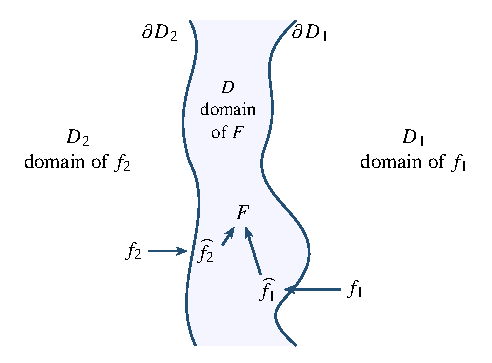
\includegraphics[width=.72\textwidth]{cd11-fig-01.pdf}
\FigureTag{CD11.1}{fig:cd11-01}
\end{figure}
% Source page 2
Two questions arise:
\begin{enumerate}
\setcounter{enumi}{0}\item Can \(f_i\), defined on \(D_i\), be extended with some regularity to \(\partial D_i\)?
\setcounter{enumi}{1}\item Can the maps \(\widehat f_i\) on \(\partial D_i\) be extended to a quasiconformal map \(F\) on \(D\), whose boundary is \(\partial D_1\cup\partial D_2\)?
\end{enumerate}
If both can be answered, we can combine \(f_1,f_2\), and the gluing map \(F\) into a single quasiconformal map, provided the boundary pieces along which they agree are quasiconformally removable; finite unions of quasiarcs are a sufficient choice. Such a boundary has Lebesgue measure zero.
We introduce the objects that describe the regularity expected of boundaries and their maps in such surgery.
\setcounter{definition}{24}\begin{definition}[Quasisymmetric maps]
A map \(h:S^1\to\mathbb C\) is \emph{quasisymmetric} if it is injective and there is a strictly increasing continuous function
% Source page 3
\(\lambda:[0,\infty)\to[0,\infty)\) such that
\[
\frac{1}{\lambda\bigl(|(z_2-z_3)/(z_1-z_2)|\bigr)}
\le\left|\frac{h(z_1)-h(z_2)}{h(z_2)-h(z_3)}\right|
\le\lambda\left(\left|\frac{z_1-z_2}{z_2-z_3}\right|\right)
\]
for all distinct \(z_1,z_2,z_3\in S^1\).
\end{definition}
\setcounter{example}{0}\begin{example}
A $C^1$-diffeomorphism $h:S^1\to h(S^1)\subset\mathbb C$ is quasisymmetric. It is enough to prove that $H(t):=h(e^{2\pi it})$, regarded as a map on $\mathbb R/\mathbb Z$, is bi-Lipschitz. Put
\[
\delta(x,y):=|e^{2\pi ix}-e^{2\pi iy}|.
\]
If
\[
\frac1k\,\delta(x,y)\le|H(x)-H(y)|\le k\,\delta(x,y),
\]
then
\[
\left|\frac{H(x)-H(y)}{H(y)-H(z)}\right|
\le k^2\frac{\delta(x,y)}{\delta(y,z)},
\]
and similarly the ratio is at least $k^{-2}\delta(x,y)/\delta(y,z)$. Take $\lambda(t)=k^2t$.
Since $h$ is $C^1$, $H$ is $C^1$; $H'$ is continuous on $\mathbb R/\mathbb Z$, hence uniformly continuous, so $H$ is uniformly differentiable. Therefore
\[
\lim_{x\to y}\frac{|H(x)-H(y)|}{\delta(x,y)}
=\frac{|H'(y)|}{2\pi}.
\]
Thus the function
\[
G(x,y)=
\begin{cases}
\dfrac{|H(x)-H(y)|}{\delta(x,y)},&x\ne y,\\
\dfrac{|H'(x)|}{2\pi},&x=y,
\end{cases}
\qquad G:(\mathbb R/\mathbb Z)^2\to(0,\infty),
\]
is continuous and attains its extreme values. Its minimum is positive, so the required bi-Lipschitz constant $k$ exists.
\end{example}

% Source page 4
\setcounter{theorem}{40}\begin{proposition}
Let \(h_1,h_2\) be quasisymmetric maps.
\begin{enumerate}[label=(\alph*)]
\setcounter{enumi}{0}\item If \(h_1(S^1)=S^1\), then \(h_2\circ h_1\) is quasisymmetric.
\setcounter{enumi}{1}\item If \(h_1(S^1)=h_2(S^1)\), then \(h=h_2^{-1}\circ h_1\) is quasisymmetric.
\end{enumerate}
\end{proposition}
\begin{proof}
It is enough to prove the inequality on one side; exchange variables for the other. For (a),
\[
\left|\frac{h_2(h_1(x))-h_2(h_1(y))}
{h_2(h_1(y))-h_2(h_1(z))}\right|
\le\lambda_2\left(\left|\frac{h_1(x)-h_1(y)}
{h_1(y)-h_1(z)}\right|\right),
\]
and the inner ratio is at most \(\lambda_1(|(x-y)/(y-z)|)\). Combining the bounds proves (a).

For (b), set
\(\lambda=(1/z)\circ\lambda_2^{-1}\circ(1/z)\circ\lambda_1\), or
\[
\lambda(t)=\frac1{\lambda_2^{-1}(1/\lambda_1(t))}.
\]
This function is strictly increasing. The inequalities for \(h_2\) and its injectivity give
\[
\frac1{\lambda_2\!\left(
\left|\frac{h_2^{-1}(x)-h_2^{-1}(y)}
{h_2^{-1}(y)-h_2^{-1}(z)}\right|^{-1}\right)}
\le\left|\frac{x-y}{y-z}\right|
\le\lambda_2\!\left(
\left|\frac{h_2^{-1}(x)-h_2^{-1}(y)}
{h_2^{-1}(y)-h_2^{-1}(z)}\right|\right).
\]
Substituting \(h_1(x),h_1(y),h_1(z)\) yields
\[
\frac1{\lambda_2\!\left(
\left|\frac{h(x)-h(y)}{h(y)-h(z)}\right|^{-1}\right)}
\le\left|\frac{h_1(x)-h_1(y)}{h_1(y)-h_1(z)}\right|
\le\lambda_2\!\left(\left|\frac{h(x)-h(y)}{h(y)-h(z)}\right|\right).
\]
% Source page 5
In particular,
\[
\frac1{\lambda_2\!\left(
\left|\frac{h(y)-h(z)}{h(x)-h(y)}\right|\right)}
\le\left|\frac{h_1(x)-h_1(y)}{h_1(y)-h_1(z)}\right|
\le\lambda_1\left(\left|\frac{x-y}{y-z}\right|\right).
\]
Hence
\[
\frac1{\lambda_1(|(x-y)/(y-z)|)}
\le\lambda_2\left(\left|\frac{h(y)-h(z)}{h(x)-h(y)}\right|\right).
\]
Since \(\lambda_2\) is increasing, applying its inverse gives
\[
\lambda_2^{-1}\left(\frac1{\lambda_1(|(x-y)/(y-z)|)}\right)
\le\left|\frac{h(y)-h(z)}{h(x)-h(y)}\right|,
\]
which is equivalent to the required upper bound by \(\lambda\).
\end{proof}
\setcounter{definition}{25}\begin{definition}[Quasiarcs]
A Jordan arc \(\gamma\) is a \emph{quasiarc} if there is \(c>0\) such that
\[
\operatorname{diam}\bigl(\gamma[z_1,z_2]\bigr)\le c|z_1-z_2|
\qquad(z_1,z_2\in\gamma).
\]
A Jordan curve satisfying the analogous inequality for the smaller subarc between every pair of points is called a \emph{quasicircle}.
\end{definition}
We now state two theorems connecting these objects for the unit disc; they will serve as models for other domains.

% Source page 6
\setcounter{theorem}{41}\begin{theorem}[Domain to boundary]\label{thm:cd11-domain-boundary}
Let \(G\) be a Jordan domain, \(\gamma=\partial G\), and \(f:\mathbb D\to G\) a conformal isomorphism. Then \(f\) has a quasisymmetric extension to \(S^1\) if and only if \(\gamma\) is a quasicircle. That is, there exists \(\widetilde f:\overline{\mathbb D}\to\overline G\) with \(\widetilde f|_{\mathbb D}=f\) and \(\widetilde f|_{S^1}=\widehat f\) quasisymmetric.
\end{theorem}
\setcounter{theorem}{42}\begin{theorem}[Boundary to domain]\label{thm:cd11-boundary-domain}
Every orientation-preserving quasisymmetric homeomorphism \(f:S^1\to S^1\) extends to \(\widehat f:\overline{\mathbb D}\to\overline{\mathbb D}\) whose restriction to \(\mathbb D\) is quasiconformal.
\end{theorem}
These theorems guide the quasiconformal filling of a domain by interpolation of its boundary maps. First we address the boundary-extension question, whose answer is as satisfying as Carath\'eodory's conformal extension theorem.
\setcounter{theorem}{43}\begin{proposition}
A quasiconformal map \(f:\mathbb H\to\mathbb H\) extends continuously to its boundary.
\end{proposition}
% Source page 7
\begin{proof}
Let $\mu_f$ be the pullback of the circle field on $\mathbb H$ via $f$.
Define
\[
\mu(z)=
\begin{cases}
\mu_f(z),&z\in\mathbb H,\\
\overline{\mu_f(\bar z)},&z\in-\mathbb H,\\
0,&z\in\mathbb R.
\end{cases}
\]
This is measurable and essentially bounded with norm strictly below one.
By the measurable Riemann mapping theorem, there is
$\varphi:\widehat{\mathbb C}\to\widehat{\mathbb C}$ pulling $\mu$ back
from the circle field. Normalize $\varphi(0)=0$, $\varphi(1)=1$, and
$\varphi(\infty)=\infty$, and put $g(z)=\overline{\varphi(\bar z)}$.
Then
\[
\frac{\partial_{\bar z}(\varphi\circ g^{-1})}
{\partial_z(\varphi\circ g^{-1})}=0,
\]
either by explicitly computing the complex dilatation or by following
the circle field. Thus $\varphi\circ g^{-1}$ is holomorphic and a
homeomorphism: a conformal automorphism fixing zero, one, and infinity.
It equals the identity, so $\varphi=g$, and
$\varphi(\mathbb R)=\mathbb R$.

Now $h=f\circ(\varphi|_{\mathbb H})^{-1}:\mathbb H\to\mathbb H$ is
conformal by Weyl's lemma. As a conformal automorphism of $\mathbb H$,
$h$ is a M\"obius map with real coefficients and therefore has a
continuous extension
$\widehat h:\overline{\mathbb H}\to\overline{\mathbb H}$ on the Riemann
sphere. Then
$\widehat f=\widehat h\circ\varphi|_{\overline{\mathbb H}}$ is the
required extension.
\end{proof}

% Source page 8
We can therefore formulate Carath\'eodory's theorem for quasiconformal maps.
\setcounter{theorem}{44}\begin{theorem}
If \(f:\mathbb D\to G\) is quasiconformal and \(G\) is a Jordan domain, then \(f\) extends continuously to the boundary.
\end{theorem}
\begin{proof}
A Riemann map \(\varphi:\mathbb D\to G\) extends continuously to \(S^1\) by Carath\'eodory's theorem. By the preceding proposition, \(\varphi^{-1}\circ f\) also extends to \(S^1\). Combining the extensions proves the claim.
\end{proof}
When $G$ is a quasidisc, one can in fact prove that \(f:\mathbb D\to G\) extends quasisymmetrically to \(S^1\). Working with this boundary regularity is therefore rather forced.

We need analogues of Theorems~\ref{thm:cd11-domain-boundary} and~\ref{thm:cd11-boundary-domain} for domains other than \(\mathbb D\). General domains are difficult because we lack tools to capture all their analytic qualities. Extension constructions use many of those qualities, especially in choosing covering spaces. We illustrate the ideas for an annulus; such results provide partial answers to the initial questions.

% Source page 9
\setcounter{theorem}{45}\begin{theorem}[Annulus: domain to boundary]
Put \(A_r=\{z:r<|z|<1\}\). Let \(A\) be a Jordan annulus and \(f:A_r\to A\) a conformal isomorphism. If \(\gamma^i,\gamma^o\) are its inner and outer boundaries, then \(f\) extends quasisymmetrically to both \(S^1\) and \(S_r^1=\{z:|z|=r\}\) if and only if both \(\gamma^i,\gamma^o\) are quasicircles.
\end{theorem}
\begin{proof}
First, the picture:
\begin{figure}[H]\centering
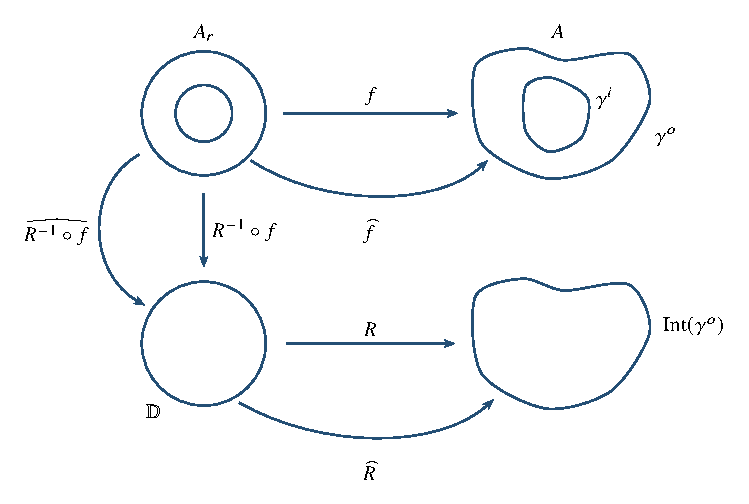
\includegraphics[width=.83\textwidth]{cd11-fig-02.pdf}
\FigureTag{CD11.2}{fig:cd11-02}
\end{figure}
Let \(R:\mathbb D\to\operatorname{Int}(\gamma^o)\) be a Riemann map. Then \(R^{-1}\circ f:A_r\to\mathbb D\).
% Source page 10
Schwarz reflection extends this to \(A_{r,1/r}=\{z:r<|z|<1/r\}\), so its restriction to \(S^1\) is analytic.
Let \(b=(R^{-1}\circ f)|_{S^1}\) and set \(\widehat f=\widehat R\circ b\), where \(\widehat R\) is the boundary extension of \(R\). Then
\[
\widehat f\text{ is quasisymmetric}
\ \Longleftrightarrow\
\widehat R\text{ is quasisymmetric}
\ \Longleftrightarrow\
\gamma^o\text{ is a quasicircle}.
\]
Using the exterior domain of \(\gamma^i\) in \(\widehat{\mathbb C}\) similarly proves the corresponding statement for the inner boundary.
\end{proof}
\setcounter{theorem}{46}\begin{theorem}[Annulus: boundary to domain]
Let \(0<r_1,r_2<1\). Two orientation-preserving quasisymmetric homeomorphisms
\(f_1:S^1\to S^1\) and \(f_2:S_{r_1}^1\to S_{r_2}^1\) extend to a map
\(f:\overline{A_{r_1}}\to\overline{A_{r_2}}\) whose restriction to \(A_{r_1}\) is quasiconformal.
\end{theorem}
\begin{proof}
This requires considerably more construction. First introduce the \emph{Beurling--Ahlfors extension} \(Bf\) of a quasisymmetric map \(f:\mathbb R\to\mathbb R\) to \(\mathbb H\).
% Source page 11
It is given in the notes by
\[
Bf(x+iy)=\frac12\int_0^1\bigl(f(x+ty)+f(x-ty)\bigr)\,dt
+i\int_0^1\bigl(f(x+ty)-f(x-ty)\bigr)\,dt.
\]
Equivalently, the notes write
\[
Bf(x+iy)=\frac1{2y}\int_{x-y}^{x+y}f(s)\,ds
+\frac{i}{y}\left(\int_x^{x+y}f(s)\,ds-\int_{x-y}^{x}f(s)\,ds\right).
\]
Since \(f\) is continuous, write the derivatives as
\[
\begin{aligned}
\frac{\partial Bf}{\partial x}
&=\underbrace{\frac{f(x+y)-f(x-y)}{2y}}_A
+i\underbrace{\frac{(f(x+y)-f(x))-(f(x)-f(x-y))}{y}}_B,\\
\frac{\partial Bf}{\partial y}
&=\underbrace{-\frac1{2y^2}\int_{x-y}^{x+y}f(s)\,ds}_C
+i\underbrace{-\frac1{y^2}
\left(\int_x^{x+y}f(s)\,ds-\int_{x-y}^{x}f(s)\,ds\right)}_D\\
&\quad+\underbrace{\frac{f(x+y)+f(x-y)}{2y}}_E
+i\underbrace{\frac{f(x+y)-f(x-y)}y}_F.
\end{aligned}
\]
Thus
\[
\begin{aligned}
\frac{\partial_{\bar z}(Bf)}{\partial_z(Bf)}
&=\frac{(Bf)_x+i(Bf)_y}{(Bf)_x-i(Bf)_y}
=\frac{A+iB+i(C+iD+E+iF)}{A+iB-i(C+iD+E+iF)}\\
&=\frac{(A-D-F)+i(B+C+E)}
{(A+D+F)+i(B-C-E)}.
\end{aligned}
\]
The preceding computation is used to establish the following bound for some $k<1$ depending only on the quasisymmetry function:
\[
\left|\frac{\partial_{\bar z}(Bf)}{\partial_z(Bf)}\right|\le k<1.
\]
One convenient quantitative form of the estimate that leads to this is
\[
|A|+|B|=O\bigl(|A+D+F|+|B-C-E|\bigr).
\]
This last bound follows from quasisymmetry.

% Source page 12
If \(f\) lifts a quasisymmetric circle homeomorphism, then \(f(x+1)=f(x)+1\). One checks that \(Bf(x+i)\) has imaginary part one, so \(\{z:\operatorname{Im}z=1\}\) is invariant under \(Bf\); this will be crucial.
If \(f(x)=x+\theta(x)\), then the real part of \(Bf\) on this line is \(x+\alpha\), where \(\alpha=\int_0^1\theta(t)\,dt\).

Return to the main problem. Lift \(\overline{A_{r_i}}\) to
\(\Sigma_3=\{z:0\le\operatorname{Im}z\le3\}\). Let
\(\Pi_{r_i}:\Sigma_3\to\overline{A_{r_i}}\) be the projections. These are holomorphic covering maps: essentially exponential conformal maps composed with a scaling factor.
Lift \(f_1,f_2\) to \(F_1,F_2\) and set
\[
\widetilde F_1=F_1,\qquad \widetilde F_2=F_2-3i,\qquad
\widetilde F_j(x)=x+\theta_j(x),\quad
\alpha_j=\int_0^1\theta_j(t)\,dt.
\]
\begin{figure}[H]\centering
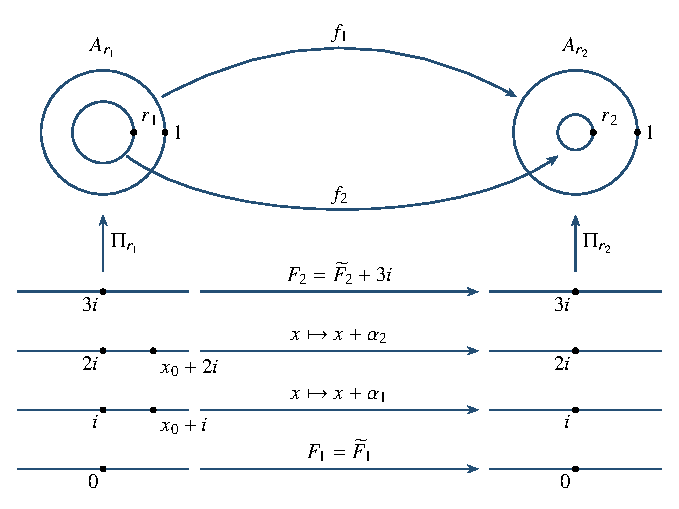
\includegraphics[width=.88\textwidth]{cd11-fig-03.pdf}
\FigureTag{CD11.3}{fig:cd11-03}
\end{figure}

% Source page 13
The ingenious step is to divide \(\Sigma_3\) into
\[
\Sigma_1=\{0\le\operatorname{Im}z\le1\},\quad
\Sigma_{1,2}=\{1\le\operatorname{Im}z\le2\},\quad
\Sigma_{2,3}=\{2\le\operatorname{Im}z\le3\}.
\]
On \(\Sigma_1\), define the extension to be \(B\widetilde F_1\). As above, its restriction to the upper edge is \(z\mapsto z+\alpha_1\).
\begin{figure}[H]\centering
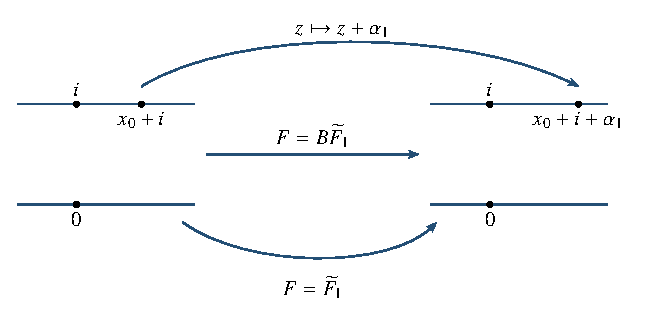
\includegraphics[width=.81\textwidth]{cd11-fig-04.pdf}
\FigureTag{CD11.4}{fig:cd11-04}
\end{figure}
Next, turn \(\Sigma_{2,3}\) around, paste it onto \(\Sigma_1\), and define its extension as already done there.
\begin{figure}[H]\centering
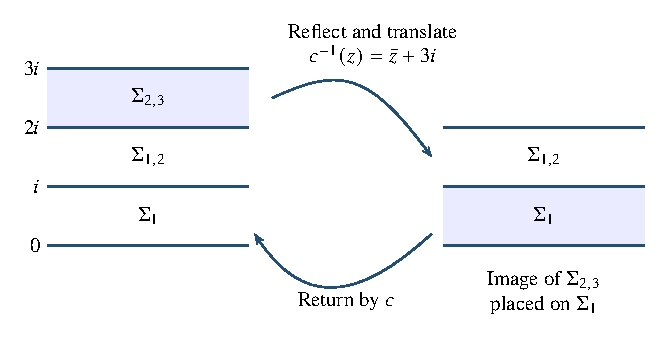
\includegraphics[width=.82\textwidth]{cd11-fig-05.pdf}
\FigureTag{CD11.5}{fig:cd11-05}
\end{figure}

% Source page 14
Mathematically, put
\[
F=c\circ B\widetilde F_2\circ c^{-1},
\qquad c(z)=\bar z+3i.
\]
Then \(F(x+2i)=x+\alpha_2+2i\). The figure shows the two extensions on the outer strips:
\begin{figure}[H]\centering
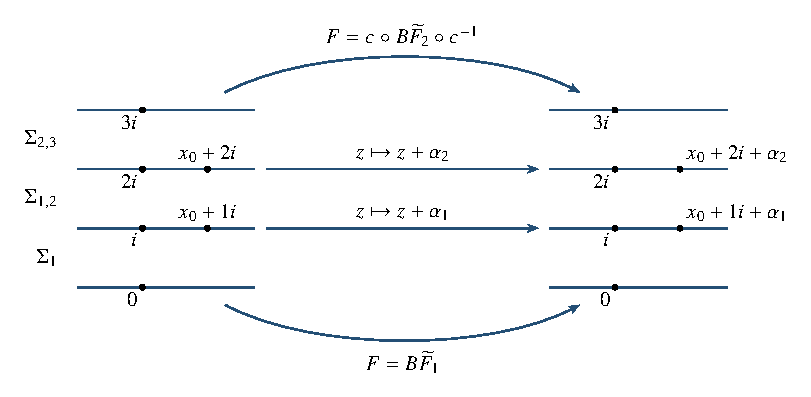
\includegraphics[width=.88\textwidth]{cd11-fig-06.pdf}
\FigureTag{CD11.6}{fig:cd11-06}
\end{figure}
On \(\partial\Sigma_{1,2}\), \(F\) acts by affine translations. Extension across the middle strip is now easy:
\begin{figure}[H]\centering
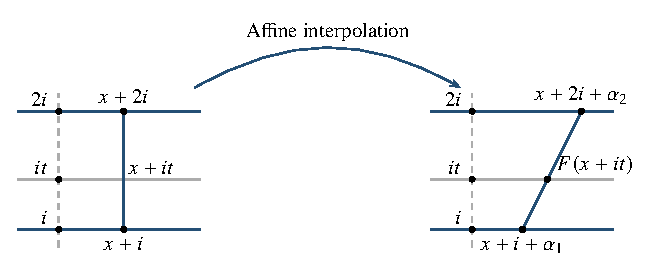
\includegraphics[width=.84\textwidth]{cd11-fig-07.pdf}
\FigureTag{CD11.7}{fig:cd11-07}
\end{figure}
Write \(\operatorname{Im}z=1+t\), \(0\le t\le1\). As these lines approach either boundary, the map must become \(x\mapsto x+\alpha_1+i\) or \(x\mapsto x+\alpha_2+2i\). Intermediate maps are given by the straight-line homotopy joining the boundary maps, viewed as loops around infinity.

% Source page 15
Explicitly, the notes give
\[
F(x+i(1+t))
=(1-t)(B\widetilde F_1)(x+i)
+t(c\circ B\widetilde F_2\circ c^{-1})(x+2i).
\]
It follows that \(F\) on \(\Sigma_{1,2}\) is \(C^1\). Direct differentiation shows that its Jacobian is positive and its Beltrami coefficient has norm strictly below one; hence it is quasiconformal.
The combined map satisfies \(F(z+1)=F(z)+1\), so it projects to the required quasiconformal map
\(f:\overline{A_{r_1}}\to\overline{A_{r_2}}\).
\end{proof}
% BLOG-CONTENT-END
\end{document}
